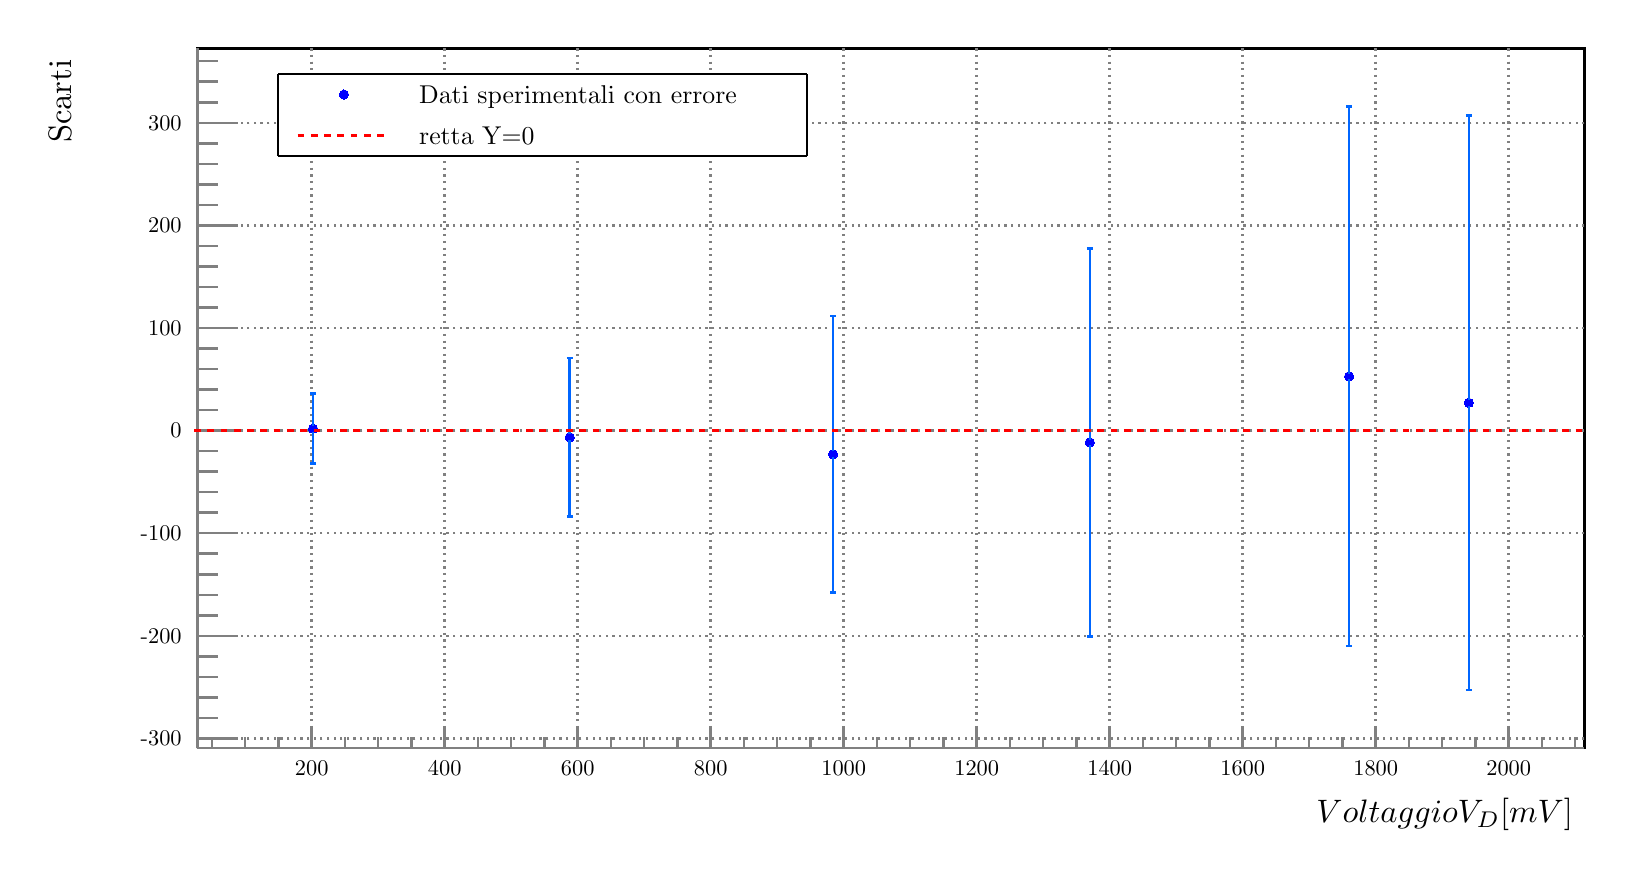
\begin{tikzpicture}
\pgfdeclareplotmark{cross} {
\pgfpathmoveto{\pgfpoint{-0.3\pgfplotmarksize}{\pgfplotmarksize}}
\pgfpathlineto{\pgfpoint{+0.3\pgfplotmarksize}{\pgfplotmarksize}}
\pgfpathlineto{\pgfpoint{+0.3\pgfplotmarksize}{0.3\pgfplotmarksize}}
\pgfpathlineto{\pgfpoint{+1\pgfplotmarksize}{0.3\pgfplotmarksize}}
\pgfpathlineto{\pgfpoint{+1\pgfplotmarksize}{-0.3\pgfplotmarksize}}
\pgfpathlineto{\pgfpoint{+0.3\pgfplotmarksize}{-0.3\pgfplotmarksize}}
\pgfpathlineto{\pgfpoint{+0.3\pgfplotmarksize}{-1.\pgfplotmarksize}}
\pgfpathlineto{\pgfpoint{-0.3\pgfplotmarksize}{-1.\pgfplotmarksize}}
\pgfpathlineto{\pgfpoint{-0.3\pgfplotmarksize}{-0.3\pgfplotmarksize}}
\pgfpathlineto{\pgfpoint{-1.\pgfplotmarksize}{-0.3\pgfplotmarksize}}
\pgfpathlineto{\pgfpoint{-1.\pgfplotmarksize}{0.3\pgfplotmarksize}}
\pgfpathlineto{\pgfpoint{-0.3\pgfplotmarksize}{0.3\pgfplotmarksize}}
\pgfpathclose
\pgfusepathqstroke
}
\pgfdeclareplotmark{cross*} {
\pgfpathmoveto{\pgfpoint{-0.3\pgfplotmarksize}{\pgfplotmarksize}}
\pgfpathlineto{\pgfpoint{+0.3\pgfplotmarksize}{\pgfplotmarksize}}
\pgfpathlineto{\pgfpoint{+0.3\pgfplotmarksize}{0.3\pgfplotmarksize}}
\pgfpathlineto{\pgfpoint{+1\pgfplotmarksize}{0.3\pgfplotmarksize}}
\pgfpathlineto{\pgfpoint{+1\pgfplotmarksize}{-0.3\pgfplotmarksize}}
\pgfpathlineto{\pgfpoint{+0.3\pgfplotmarksize}{-0.3\pgfplotmarksize}}
\pgfpathlineto{\pgfpoint{+0.3\pgfplotmarksize}{-1.\pgfplotmarksize}}
\pgfpathlineto{\pgfpoint{-0.3\pgfplotmarksize}{-1.\pgfplotmarksize}}
\pgfpathlineto{\pgfpoint{-0.3\pgfplotmarksize}{-0.3\pgfplotmarksize}}
\pgfpathlineto{\pgfpoint{-1.\pgfplotmarksize}{-0.3\pgfplotmarksize}}
\pgfpathlineto{\pgfpoint{-1.\pgfplotmarksize}{0.3\pgfplotmarksize}}
\pgfpathlineto{\pgfpoint{-0.3\pgfplotmarksize}{0.3\pgfplotmarksize}}
\pgfpathclose
\pgfusepathqfillstroke
}
\pgfdeclareplotmark{newstar} {
\pgfpathmoveto{\pgfqpoint{0pt}{\pgfplotmarksize}}
\pgfpathlineto{\pgfqpointpolar{44}{0.5\pgfplotmarksize}}
\pgfpathlineto{\pgfqpointpolar{18}{\pgfplotmarksize}}
\pgfpathlineto{\pgfqpointpolar{-20}{0.5\pgfplotmarksize}}
\pgfpathlineto{\pgfqpointpolar{-54}{\pgfplotmarksize}}
\pgfpathlineto{\pgfqpointpolar{-90}{0.5\pgfplotmarksize}}
\pgfpathlineto{\pgfqpointpolar{234}{\pgfplotmarksize}}
\pgfpathlineto{\pgfqpointpolar{198}{0.5\pgfplotmarksize}}
\pgfpathlineto{\pgfqpointpolar{162}{\pgfplotmarksize}}
\pgfpathlineto{\pgfqpointpolar{134}{0.5\pgfplotmarksize}}
\pgfpathclose
\pgfusepathqstroke
}
\pgfdeclareplotmark{newstar*} {
\pgfpathmoveto{\pgfqpoint{0pt}{\pgfplotmarksize}}
\pgfpathlineto{\pgfqpointpolar{44}{0.5\pgfplotmarksize}}
\pgfpathlineto{\pgfqpointpolar{18}{\pgfplotmarksize}}
\pgfpathlineto{\pgfqpointpolar{-20}{0.5\pgfplotmarksize}}
\pgfpathlineto{\pgfqpointpolar{-54}{\pgfplotmarksize}}
\pgfpathlineto{\pgfqpointpolar{-90}{0.5\pgfplotmarksize}}
\pgfpathlineto{\pgfqpointpolar{234}{\pgfplotmarksize}}
\pgfpathlineto{\pgfqpointpolar{198}{0.5\pgfplotmarksize}}
\pgfpathlineto{\pgfqpointpolar{162}{\pgfplotmarksize}}
\pgfpathlineto{\pgfqpointpolar{134}{0.5\pgfplotmarksize}}
\pgfpathclose
\pgfusepathqfillstroke
}
\definecolor{c}{rgb}{1,1,1};
\draw [color=c, fill=c] (0,0) rectangle (20,10.4736);
\draw [color=c, fill=c] (2.14936,1.32969) rectangle (19.7632,10.2186);
\definecolor{c}{rgb}{0,0,0};
\draw [c,line width=0.9] (2.14936,1.32969) -- (2.14936,10.2186) -- (19.7632,10.2186) -- (19.7632,1.32969) -- (2.14936,1.32969);
\definecolor{c}{rgb}{1,1,1};
\draw [color=c, fill=c] (2.14936,1.32969) rectangle (19.7632,10.2186);
\definecolor{c}{rgb}{0,0,0};
\draw [c,line width=0.9] (2.14936,1.32969) -- (2.14936,10.2186) -- (19.7632,10.2186) -- (19.7632,1.32969) -- (2.14936,1.32969);
\definecolor{c}{rgb}{0.5,0.5,0.5};
\draw [c,line width=0.9] (2.14936,1.32969) -- (19.7632,1.32969);
\draw [c,dash pattern=on 0.80pt off 1.60pt ,line width=0.9] (3.60029,10.2186) -- (3.60029,1.32969);
\draw [c,dash pattern=on 0.80pt off 1.60pt ,line width=0.9] (5.28938,10.2186) -- (5.28938,1.32969);
\draw [c,dash pattern=on 0.80pt off 1.60pt ,line width=0.9] (6.97847,10.2186) -- (6.97847,1.32969);
\draw [c,dash pattern=on 0.80pt off 1.60pt ,line width=0.9] (8.66757,10.2186) -- (8.66757,1.32969);
\draw [c,dash pattern=on 0.80pt off 1.60pt ,line width=0.9] (10.3567,10.2186) -- (10.3567,1.32969);
\draw [c,dash pattern=on 0.80pt off 1.60pt ,line width=0.9] (12.0457,10.2186) -- (12.0457,1.32969);
\draw [c,dash pattern=on 0.80pt off 1.60pt ,line width=0.9] (13.7348,10.2186) -- (13.7348,1.32969);
\draw [c,dash pattern=on 0.80pt off 1.60pt ,line width=0.9] (15.4239,10.2186) -- (15.4239,1.32969);
\draw [c,dash pattern=on 0.80pt off 1.60pt ,line width=0.9] (17.113,10.2186) -- (17.113,1.32969);
\draw [c,dash pattern=on 0.80pt off 1.60pt ,line width=0.9] (18.8021,10.2186) -- (18.8021,1.32969);
\draw [c,dash pattern=on 0.80pt off 1.60pt ,line width=0.9] (3.60029,10.2186) -- (3.60029,1.32969);
\draw [c,dash pattern=on 0.80pt off 1.60pt ,line width=0.9] (18.8021,10.2186) -- (18.8021,1.32969);
\draw [c,line width=0.9] (2.14936,1.32969) -- (2.14936,10.2186);
\draw [c,dash pattern=on 0.80pt off 1.60pt ,line width=0.9] (19.7632,1.45393) -- (2.14936,1.45393);
\draw [c,dash pattern=on 0.80pt off 1.60pt ,line width=0.9] (19.7632,2.75704) -- (2.14936,2.75704);
\draw [c,dash pattern=on 0.80pt off 1.60pt ,line width=0.9] (19.7632,4.06016) -- (2.14936,4.06016);
\draw [c,dash pattern=on 0.80pt off 1.60pt ,line width=0.9] (19.7632,5.36328) -- (2.14936,5.36328);
\draw [c,dash pattern=on 0.80pt off 1.60pt ,line width=0.9] (19.7632,6.66639) -- (2.14936,6.66639);
\draw [c,dash pattern=on 0.80pt off 1.60pt ,line width=0.9] (19.7632,7.96951) -- (2.14936,7.96951);
\draw [c,dash pattern=on 0.80pt off 1.60pt ,line width=0.9] (19.7632,9.27262) -- (2.14936,9.27262);
\draw [c,dash pattern=on 0.80pt off 1.60pt ,line width=0.9] (19.7632,1.45393) -- (2.14936,1.45393);
\draw [c,dash pattern=on 0.80pt off 1.60pt ,line width=0.9] (19.7632,9.27262) -- (2.14936,9.27262);
\draw [c,line width=0.9] (2.14936,1.32969) -- (19.7632,1.32969);
\draw [c,line width=0.9] (3.60029,1.60641) -- (3.60029,1.32969);
\draw [c,line width=0.9] (4.02256,1.46805) -- (4.02256,1.32969);
\draw [c,line width=0.9] (4.44484,1.46805) -- (4.44484,1.32969);
\draw [c,line width=0.9] (4.86711,1.46805) -- (4.86711,1.32969);
\draw [c,line width=0.9] (5.28938,1.60641) -- (5.28938,1.32969);
\draw [c,line width=0.9] (5.71166,1.46805) -- (5.71166,1.32969);
\draw [c,line width=0.9] (6.13393,1.46805) -- (6.13393,1.32969);
\draw [c,line width=0.9] (6.5562,1.46805) -- (6.5562,1.32969);
\draw [c,line width=0.9] (6.97847,1.60641) -- (6.97847,1.32969);
\draw [c,line width=0.9] (7.40075,1.46805) -- (7.40075,1.32969);
\draw [c,line width=0.9] (7.82302,1.46805) -- (7.82302,1.32969);
\draw [c,line width=0.9] (8.24529,1.46805) -- (8.24529,1.32969);
\draw [c,line width=0.9] (8.66757,1.60641) -- (8.66757,1.32969);
\draw [c,line width=0.9] (9.08984,1.46805) -- (9.08984,1.32969);
\draw [c,line width=0.9] (9.51211,1.46805) -- (9.51211,1.32969);
\draw [c,line width=0.9] (9.93438,1.46805) -- (9.93438,1.32969);
\draw [c,line width=0.9] (10.3567,1.60641) -- (10.3567,1.32969);
\draw [c,line width=0.9] (10.7789,1.46805) -- (10.7789,1.32969);
\draw [c,line width=0.9] (11.2012,1.46805) -- (11.2012,1.32969);
\draw [c,line width=0.9] (11.6235,1.46805) -- (11.6235,1.32969);
\draw [c,line width=0.9] (12.0457,1.60641) -- (12.0457,1.32969);
\draw [c,line width=0.9] (12.468,1.46805) -- (12.468,1.32969);
\draw [c,line width=0.9] (12.8903,1.46805) -- (12.8903,1.32969);
\draw [c,line width=0.9] (13.3126,1.46805) -- (13.3126,1.32969);
\draw [c,line width=0.9] (13.7348,1.60641) -- (13.7348,1.32969);
\draw [c,line width=0.9] (14.1571,1.46805) -- (14.1571,1.32969);
\draw [c,line width=0.9] (14.5794,1.46805) -- (14.5794,1.32969);
\draw [c,line width=0.9] (15.0017,1.46805) -- (15.0017,1.32969);
\draw [c,line width=0.9] (15.4239,1.60641) -- (15.4239,1.32969);
\draw [c,line width=0.9] (15.8462,1.46805) -- (15.8462,1.32969);
\draw [c,line width=0.9] (16.2685,1.46805) -- (16.2685,1.32969);
\draw [c,line width=0.9] (16.6907,1.46805) -- (16.6907,1.32969);
\draw [c,line width=0.9] (17.113,1.60641) -- (17.113,1.32969);
\draw [c,line width=0.9] (17.5353,1.46805) -- (17.5353,1.32969);
\draw [c,line width=0.9] (17.9576,1.46805) -- (17.9576,1.32969);
\draw [c,line width=0.9] (18.3798,1.46805) -- (18.3798,1.32969);
\draw [c,line width=0.9] (18.8021,1.60641) -- (18.8021,1.32969);
\draw [c,line width=0.9] (3.60029,1.60641) -- (3.60029,1.32969);
\draw [c,line width=0.9] (3.17802,1.46805) -- (3.17802,1.32969);
\draw [c,line width=0.9] (2.75575,1.46805) -- (2.75575,1.32969);
\draw [c,line width=0.9] (2.33347,1.46805) -- (2.33347,1.32969);
\draw [c,line width=0.9] (18.8021,1.60641) -- (18.8021,1.32969);
\draw [c,line width=0.9] (19.2244,1.46805) -- (19.2244,1.32969);
\draw [c,line width=0.9] (19.6467,1.46805) -- (19.6467,1.32969);
\definecolor{c}{rgb}{0,0,0};
\draw [anchor=base] (3.60029,0.984062) node[scale=0.809097, color=c, rotate=0]{200};
\draw [anchor=base] (5.28938,0.984062) node[scale=0.809097, color=c, rotate=0]{400};
\draw [anchor=base] (6.97847,0.984062) node[scale=0.809097, color=c, rotate=0]{600};
\draw [anchor=base] (8.66757,0.984062) node[scale=0.809097, color=c, rotate=0]{800};
\draw [anchor=base] (10.3567,0.984062) node[scale=0.809097, color=c, rotate=0]{1000};
\draw [anchor=base] (12.0457,0.984062) node[scale=0.809097, color=c, rotate=0]{1200};
\draw [anchor=base] (13.7348,0.984062) node[scale=0.809097, color=c, rotate=0]{1400};
\draw [anchor=base] (15.4239,0.984062) node[scale=0.809097, color=c, rotate=0]{1600};
\draw [anchor=base] (17.113,0.984062) node[scale=0.809097, color=c, rotate=0]{1800};
\draw [anchor=base] (18.8021,0.984062) node[scale=0.809097, color=c, rotate=0]{2000};
\draw [anchor= east] (19.7632,0.491803) node[scale=1.17319, color=c, rotate=0]{$Voltaggio V_{D} [mV]$};
\definecolor{c}{rgb}{0.5,0.5,0.5};
\draw [c,line width=0.9] (2.14936,1.32969) -- (2.14936,10.2186);
\draw [c,line width=0.9] (2.65858,1.45393) -- (2.14936,1.45393);
\draw [c,line width=0.9] (2.40397,1.71455) -- (2.14936,1.71455);
\draw [c,line width=0.9] (2.40397,1.97517) -- (2.14936,1.97517);
\draw [c,line width=0.9] (2.40397,2.2358) -- (2.14936,2.2358);
\draw [c,line width=0.9] (2.40397,2.49642) -- (2.14936,2.49642);
\draw [c,line width=0.9] (2.65858,2.75704) -- (2.14936,2.75704);
\draw [c,line width=0.9] (2.40397,3.01767) -- (2.14936,3.01767);
\draw [c,line width=0.9] (2.40397,3.27829) -- (2.14936,3.27829);
\draw [c,line width=0.9] (2.40397,3.53891) -- (2.14936,3.53891);
\draw [c,line width=0.9] (2.40397,3.79954) -- (2.14936,3.79954);
\draw [c,line width=0.9] (2.65858,4.06016) -- (2.14936,4.06016);
\draw [c,line width=0.9] (2.40397,4.32078) -- (2.14936,4.32078);
\draw [c,line width=0.9] (2.40397,4.58141) -- (2.14936,4.58141);
\draw [c,line width=0.9] (2.40397,4.84203) -- (2.14936,4.84203);
\draw [c,line width=0.9] (2.40397,5.10265) -- (2.14936,5.10265);
\draw [c,line width=0.9] (2.65858,5.36328) -- (2.14936,5.36328);
\draw [c,line width=0.9] (2.40397,5.6239) -- (2.14936,5.6239);
\draw [c,line width=0.9] (2.40397,5.88452) -- (2.14936,5.88452);
\draw [c,line width=0.9] (2.40397,6.14515) -- (2.14936,6.14515);
\draw [c,line width=0.9] (2.40397,6.40577) -- (2.14936,6.40577);
\draw [c,line width=0.9] (2.65858,6.66639) -- (2.14936,6.66639);
\draw [c,line width=0.9] (2.40397,6.92701) -- (2.14936,6.92701);
\draw [c,line width=0.9] (2.40397,7.18764) -- (2.14936,7.18764);
\draw [c,line width=0.9] (2.40397,7.44826) -- (2.14936,7.44826);
\draw [c,line width=0.9] (2.40397,7.70888) -- (2.14936,7.70888);
\draw [c,line width=0.9] (2.65858,7.96951) -- (2.14936,7.96951);
\draw [c,line width=0.9] (2.40397,8.23013) -- (2.14936,8.23013);
\draw [c,line width=0.9] (2.40397,8.49075) -- (2.14936,8.49075);
\draw [c,line width=0.9] (2.40397,8.75138) -- (2.14936,8.75138);
\draw [c,line width=0.9] (2.40397,9.012) -- (2.14936,9.012);
\draw [c,line width=0.9] (2.65858,9.27262) -- (2.14936,9.27262);
\draw [c,line width=0.9] (2.65858,1.45393) -- (2.14936,1.45393);
\draw [c,line width=0.9] (2.65858,9.27262) -- (2.14936,9.27262);
\draw [c,line width=0.9] (2.40397,9.53325) -- (2.14936,9.53325);
\draw [c,line width=0.9] (2.40397,9.79387) -- (2.14936,9.79387);
\draw [c,line width=0.9] (2.40397,10.0545) -- (2.14936,10.0545);
\definecolor{c}{rgb}{0,0,0};
\draw [anchor= east] (2.04936,1.45393) node[scale=0.809097, color=c, rotate=0]{-300};
\draw [anchor= east] (2.04936,2.75704) node[scale=0.809097, color=c, rotate=0]{-200};
\draw [anchor= east] (2.04936,4.06016) node[scale=0.809097, color=c, rotate=0]{-100};
\draw [anchor= east] (2.04936,5.36328) node[scale=0.809097, color=c, rotate=0]{0};
\draw [anchor= east] (2.04936,6.66639) node[scale=0.809097, color=c, rotate=0]{100};
\draw [anchor= east] (2.04936,7.96951) node[scale=0.809097, color=c, rotate=0]{200};
\draw [anchor= east] (2.04936,9.27262) node[scale=0.809097, color=c, rotate=0]{300};
\draw [anchor= east] (0.40255,10.2186) node[scale=1.17319, color=c, rotate=90]{Scarti};
\definecolor{c}{rgb}{0,0,1};
\foreach \P in {(3.61718,5.38744), (6.87713,5.27765), (10.2215,5.06238), (13.4815,5.2132), (16.7752,6.05159), (18.2954,5.71681)}{\draw[mark options={color=c,fill=c},mark size=1.681682pt, line width=0.000000pt, mark=*] plot coordinates {\P};}
\definecolor{c}{rgb}{0,0.4,1};
\draw [c,line width=0.9] (3.61718,5.42387) -- (3.61718,5.83184);
\draw [c,line width=0.9] (3.58075,5.83184) -- (3.65361,5.83184);
\draw [c,line width=0.9] (3.61718,5.35101) -- (3.61718,4.94304);
\draw [c,line width=0.9] (3.58075,4.94304) -- (3.65361,4.94304);
\draw [c,line width=0.9] (6.87713,5.31407) -- (6.87713,6.28252);
\draw [c,line width=0.9] (6.8407,6.28252) -- (6.91356,6.28252);
\draw [c,line width=0.9] (6.87713,5.24122) -- (6.87713,4.27277);
\draw [c,line width=0.9] (6.8407,4.27277) -- (6.91356,4.27277);
\draw [c,line width=0.9] (10.2215,5.09881) -- (10.2215,6.81581);
\draw [c,line width=0.9] (10.1851,6.81581) -- (10.258,6.81581);
\draw [c,line width=0.9] (10.2215,5.02595) -- (10.2215,3.30894);
\draw [c,line width=0.9] (10.1851,3.30894) -- (10.258,3.30894);
\draw [c,line width=0.9] (13.4815,5.24963) -- (13.4815,7.6764);
\draw [c,line width=0.9] (13.445,7.6764) -- (13.5179,7.6764);
\draw [c,line width=0.9] (13.4815,5.17677) -- (13.4815,2.75001);
\draw [c,line width=0.9] (13.445,2.75001) -- (13.5179,2.75001);
\draw [c,line width=0.9] (16.7752,6.08802) -- (16.7752,9.47784);
\draw [c,line width=0.9] (16.7388,9.47784) -- (16.8116,9.47784);
\draw [c,line width=0.9] (16.7752,6.01516) -- (16.7752,2.62533);
\draw [c,line width=0.9] (16.7388,2.62533) -- (16.8116,2.62533);
\draw [c,line width=0.9] (18.2954,5.75324) -- (18.2954,9.36318);
\draw [c,line width=0.9] (18.259,9.36318) -- (18.3318,9.36318);
\draw [c,line width=0.9] (18.2954,5.68038) -- (18.2954,2.07043);
\draw [c,line width=0.9] (18.259,2.07043) -- (18.3318,2.07043);
\definecolor{c}{rgb}{1,0,0};
\draw [c,dash pattern=on 2.40pt off 2.40pt ,line width=0.9] (2.10545,5.36328) -- (19.7733,5.36328);
\definecolor{c}{rgb}{1,1,1};
\draw [color=c, fill=c] (3.1694,8.85246) rectangle (9.89071,9.89071);
\definecolor{c}{rgb}{0,0,0};
\draw [c,line width=0.9] (3.1694,8.85246) -- (9.89071,8.85246);
\draw [c,line width=0.9] (9.89071,8.85246) -- (9.89071,9.89071);
\draw [c,line width=0.9] (9.89071,9.89071) -- (3.1694,9.89071);
\draw [c,line width=0.9] (3.1694,9.89071) -- (3.1694,8.85246);
\draw [anchor=base west] (4.84973,9.51434) node[scale=0.930461, color=c, rotate=0]{Dati sperimentali con errore};
\definecolor{c}{rgb}{0,0,1};
\foreach \P in {(4.00956,9.63115)}{\draw[mark options={color=c,fill=c},mark size=1.681682pt, line width=0.000000pt, mark=*] plot coordinates {\P};}
\definecolor{c}{rgb}{0,0,0};
\draw [anchor=base west] (4.84973,8.99522) node[scale=0.930461, color=c, rotate=0]{retta Y=0};
\definecolor{c}{rgb}{1,0,0};
\draw [c,dash pattern=on 2.40pt off 2.40pt ,line width=0.9] (3.42145,9.11202) -- (4.59768,9.11202);
\end{tikzpicture}
